\documentclass[12pt]{beamer}
\usepackage{../Estilos/BeamerMAF}
\usepackage{../Estilos/ColoresLatex}
\usetheme{Dresden}
\usecolortheme{seahorse}
%\useoutertheme{default}
\setbeamercovered{invisible}
% or whatever (possibly just delete it)
\setbeamertemplate{section in toc}[sections numbered]
\setbeamertemplate{subsection in toc}[subsections numbered]
\setbeamertemplate{subsection in toc}{\leavevmode\leftskip=3.2em\rlap{\hskip-2em\inserttocsectionnumber.\inserttocsubsectionnumber}\inserttocsubsection\par}
\setbeamercolor{section in toc}{fg=blue}
\setbeamercolor{subsection in toc}{fg=blue}
\setbeamercolor{frametitle}{fg=blue}
\setbeamertemplate{caption}[numbered]

\setbeamertemplate{footline}
\beamertemplatenavigationsymbolsempty
\setbeamertemplate{headline}{}

\makeatletter
\setbeamercolor{section in foot}{bg=gray!30, fg=black!90!orange}
\setbeamercolor{subsection in foot}{bg=blue!30!yellow, fg=red}
\setbeamertemplate{footline}
{
  \leavevmode%
  \hbox{%
  \begin{beamercolorbox}[wd=.333333\paperwidth,ht=2.25ex,dp=1ex,center]{section in foot}%
    \usebeamerfont{section in foot} \insertsection
  \end{beamercolorbox}}%
  \begin{beamercolorbox}[wd=.333333\paperwidth,ht=2.25ex,dp=1ex,center]{subsection in foot}%
    \usebeamerfont{subsection in foot}  \insertsubsection
  \end{beamercolorbox}%
  \begin{beamercolorbox}[wd=.333333\paperwidth,ht=2.25ex,dp=1ex,right]{date in head/foot}%
    \usebeamerfont{date in head/foot} \insertshortdate{} \hspace*{2em}
    \insertframenumber{} / \inserttotalframenumber \hspace*{2ex} 
  \end{beamercolorbox}}%
  \vskip0pt%
\makeatother 

\makeatletter
\patchcmd{\beamer@sectionintoc}{\vskip1.5em}{\vskip0.8em}{}{}
\makeatother


\setbeamercolor{section in foot}{bg=darkspringgreen, fg=white}
\setbeamercolor{subsection in foot}{bg=persianblue, fg=white}
\setbeamercolor{date in foot}{bg=goldenrod, fg=white}

\makeatletter
\setbeamertemplate{footline}
{
\leavevmode%
\hbox{%
\begin{beamercolorbox}[wd=.333333\paperwidth,ht=2.25ex,dp=1ex,center]{section in foot}%
  \usebeamerfont{section in foot} \insertsection
\end{beamercolorbox}%
\begin{beamercolorbox}[wd=.333333\paperwidth,ht=2.25ex,dp=1ex,center]{subsection in foot}%
  \usebeamerfont{subsection in foot}  \insertsubsection
\end{beamercolorbox}%
\begin{beamercolorbox}[wd=.333333\paperwidth,ht=2.25ex,dp=1ex,right]{date in head/foot}%
  \usebeamerfont{date in head/foot} \insertshortdate{} \hspace*{1.5em}
  \insertframenumber{} / \inserttotalframenumber \hspace*{2ex} 
\end{beamercolorbox}}%
\vskip0pt%
}
\makeatother
% \usefonttheme{serif}
\resetcounteronoverlays{saveenumi}

\AtBeginDocument{\RenewCommandCopy\qty\SI}
\ExplSyntaxOn
\msg_redirect_name:nnn { siunitx } { physics-pkg } { none }
\ExplSyntaxOff

\date{}

\title{\large{Teoría Operadores Sturm-Liouville}}
\subtitle{Tema 3 - Bases completas y ortogonales}
\author{M. en C. Gustavo Contreras Mayén}


\begin{document}
\maketitle
\fontsize{14}{14}\selectfont
\spanishdecimal{.}

\section*{Contenido}
\frame[allowframebreaks]{\frametitle{Contenido} \tableofcontents[currentsection, hideallsubsections]}

\section{Operadores autoadjuntos}
\frame[allowframebreaks]{\frametitle{Temas a revisar} \tableofcontents[currentsection, hideothersubsections]}
\subsection{Introducción}

\begin{frame}
\frametitle{Relevancia de los operadores}
En el estudio de la teoría espectral de matrices, se aprende sobre el adjunto de la matriz, $\vb{A}^{\dagger}$, y el papel que juegan las matrices autoadjuntas o Hermitianas en la diagonalización.
\end{frame}
\begin{frame}
\frametitle{Nuevo concepto}
Además, se necesita el concepto del \textocolor{red}{adjunto} para discutir la existencia de soluciones al problema matricial:
\begin{align*}
\vb{y} = \vb{A} \, \vb{x}
\end{align*}
\end{frame}
\begin{frame}
\frametitle{Operadores y ED}
En el mismo sentido, uno está interesado en la existencia de soluciones de la ecuación del operador $L \, u = f$ y soluciones del correspondiente problema de valores propios.
\end{frame}
\begin{frame}
\frametitle{Operadores y ED}
El estudio de operadores lineales en un espacio de Hilbert es una generalización de lo que estudia en un curso de álgebra lineal.
\end{frame}
\begin{frame}
\frametitle{Retomando el operador Sturm-Liouville}
Así como se puede encontrar una base de vectores propios y diagonalizar matrices Hermitianas o autoadjuntas (o simétricas reales en el caso de matrices reales), veremos que el operador de Sturm-Liouville es \textocolor{blue}{autoadjunto}.
\end{frame}
\begin{frame}
\frametitle{Retomando el operador Sturm-Liouville}    
En esta parte definiremos el \textocolor{bole}{dominio} de un operador e introduciremos la noción de \textocolor{debianred}{operadores adjuntos}.
\\
\bigskip
\pause
Veremos el papel que juega el adjunto en la existencia de soluciones a la ecuación del operador $L \, u = f$.
\end{frame}

\subsection{El operador adjunto}

\begin{frame}
\frametitle{Definición}
Comenzamos definiendo el adjunto de un operador: \pause el adjunto, $L^{\dagger}$, del operador $L$ satisface:
\begin{align*}
\langle u, L \, v \rangle = \langle L^{\dagger} \, u,  v \rangle
\end{align*}
para todo $v$ en el dominio de $L$ y $u$ en el dominio de $L^{\dagger}$.
\end{frame}
\begin{frame}
\frametitle{El dominio del operador}
Aquí, el dominio de un operador diferencial $L$ es el conjunto de todos $u \in L_{\sigma}^{2} (a, b)$ que satisfacen un conjunto dado de CDF homogéneas.
\\
\bigskip
\pause
Esto se comprenderá mejor con el siguiente ejemplo.
\end{frame}
\begin{frame}
\frametitle{Ejemplo de operador adjunto}
Encuentra el adjunto de:
\begin{align*}
L = a_{2}(x) \, D^{2} + a_{1}(x) \, D + a_{0}(x)
\end{align*}
con $D = \dv*{x}$.
\end{frame}
\begin{frame}
\frametitle{Resolviendo el ejemplo de operador adjunto}    
Para encontrar el adjunto, colocamos el operador dentro de una integral. 
\\
\bigskip
\pause
Consideremos el producto interior:
\begin{align*}
\langle u , L \, v \rangle = \scaleint{5ex}_{\bs a}^{b} u (a_{2} \, \sderivada{v} + a_{1} \, \pderivada{v} + a_{0} \, v) \dd{x}
\end{align*}
\end{frame}
\begin{frame}
\frametitle{Resolviendo el ejemplo}
Tenemos que \enquote{mover} el operador $L$ de $v$ \pause y determinar qué operador está actuando sobre $u$ para preservar formalmente el producto interno.
\\
\bigskip
\pause
\end{frame}
\begin{frame}
\frametitle{Resolviendo el ejemplo}    
Para un operador simple como $L = \dv*{x}$, esto se hace fácilmente mediante la integración por partes.
\\
\bigskip
\pause
Para el operador dado en el ejemplo, necesitaremos aplicar varias integraciones por partes a los términos individuales. Consideramos cada término derivado en el integrando por separado.
\end{frame}
\begin{frame}
\frametitle{Integrando el término $a_{1}$}
Para el término $a_{1} \pderivada{v}$, integramos por partes para encontrar:
\pause
\begin{eqnarray}
\begin{aligned}[b]
\scaleint{5ex}_{\bs a}^{b} \, u(x) \, &a_{1} \, \pderivada{v}(x) \dd{x} = a_{1}(x) \, u(x) \, v(x) \eval_{a}^{b} + \\[0.5em]
&- \scaleint{5ex}_{\bs a}^{b} \big[ u(x) \, a_{1} (x) \big]^{\prime} \, v(x) \dd{x}
\end{aligned}
\label{eq:ecuacion_04_17}
\end{eqnarray}
\end{frame}
\begin{frame}
\frametitle{Integrando el término $a_{2}$}
Ahora consideremos el caso para el término $a_{2} \, \sderivada{v}$, en donde será necesario hacer dos integraciones por partes:
\pause
\begin{eqnarray*}
\begin{aligned}[b]
&\scaleint{5ex}_{\bs a}^{b} \, u(x) \, a_{2} (x) \, \sderivada{v}(x) \dd{x} = a_{2}(x) \, u(x) \, \pderivada{v}(x) \eval_{a}^{b} + \\[0.5em]
&- \scaleint{5ex}_{\bs a}^{b} \big[ u(x) \, a_{2} (x) \big]^{\prime} \, \pderivada{v}(x) \dd{x} = \end{aligned}
\end{eqnarray*}
\end{frame}
\begin{frame}
\frametitle{Integrando el término $a_{2}$}
\begin{eqnarray}
\begin{aligned}[b]
&= \bigg[ a_{2}(x) \, u(x) \, \pderivada{v}(x) - \big[ a_{2}(x) \, u(x) \big]^{\prime} \, v(x) \bigg] \eval_{a}^{b} + \\[0.5em]
&+ \scaleint{5ex}_{\bs a}^{b} \, \big[ u(x) \, a_{2} (x) \big]^{\prime \prime} \, v(x) \dd{x}
\end{aligned}
\label{eq:ecuacion_04_18}
\end{eqnarray}
\end{frame}    
\begin{frame}
\frametitle{Resultado premilinar}
Combinando estos resultados, tenemos que:
\pause
\begin{eqnarray}
\begin{aligned}[b]
\langle u , L \, v \rangle &= \pause \scaleint{5ex}_{\bs a}^{b} u (a_{2} \, \sderivada{v} + a_{1} \, \pderivada{v} + a_{0} \, v) \dd{x} = \\[0.5em] \pause
&= \bigg[ a_{1}(x) \, u(x) \, v(x) + a_{2}(x) \, u(x) \, \pderivada{v}(x) + \\[0.5em]
&- \big[ a_{2}(x) \, u(x) \big]^{\prime} \, v(x) \bigg] \eval_{a}^{b} + \\[0.5em]
&+ \scaleint{5ex}_{\bs a}^{b} \, \big[ u(x) \, a_{2} (x) \big]^{\prime \prime} \, v(x) \dd{x}
\end{aligned}
\label{eq:ecuacion_04_19}
\end{eqnarray}
\end{frame}
\begin{frame}
\frametitle{Usando las CDF}
Agregando las CDF para $v$, \pause uno tiene que determinar las CDF para $u$ tales que:
\pause
\begin{align*}
&\bigg[ a_{1}(x) \, u(x) \, v(x) + a_{2}(x) \, u(x) \, \pderivada{v}(x) + \\[0.5em]
&- \big[ a_{2}(x) \, u(x) \big]^{\prime} \, v(x) \bigg] \eval_{a}^{b} = 0
\end{align*}
\end{frame}
\begin{frame}
\frametitle{Usando las CDF}
Estos nos lleva a:
\pause
\begin{align*}
\langle u , L \, v \rangle &= \scaleint{5ex}_{\bs a}^{b}  \big[ (a_{2} \, u)^{\prime \prime} - (a_{1} \, u)^{\prime} + a_{0} \, u \big] \, v \dd{x} \\[0.5em]
&\equiv \langle L^{\dagger} \, u, v \rangle 
\end{align*}
\end{frame}
\begin{frame}
\frametitle{El operador adjunto}
Por lo tanto:
\pause
\begin{align}
L^{\dagger} = a_{2}(x) \, \dv[2]{x} - a_{1}(x) \, \dv{x} + a_{0}(x)
\label{eq:ecuacion_04_20}
\end{align}
\end{frame}
\begin{frame}
\frametitle{El operador Hermitiano/Hermítico}
Cuando $L^{\dagger} = L$, \pause el operador se llama formalmente \textocolor{darkorchid}{autoadjunto}, también es conocido como \textocolor{darkred}{operador Hermitiano}.
\\
\bigskip
\pause
Cuando el dominio de $L$ es el mismo que el dominio de $L^{\dagger}$, se utiliza el término autoadjunto.
\end{frame}
\begin{frame}
\frametitle{Ejemplo 2}
Determina $L^{\dagger}$ y su dominio para el operador:
\pause
\begin{align*}
L \, u = \dv{u}{x}
\end{align*}
donde $u$ satisface las CDF $u(0) = 2 \, u(1)$ en $[0, 1]$.
\end{frame}
\begin{frame}
\frametitle{Resolviendo el ejercicio 2}
Necesitamos encontrar el operador adjunto que satisfaga $\langle v, L \, u \rangle = \langle L^{\dagger} \, v, u \rangle$.
\\
\bigskip
\pause  
Por lo que reescribimos la integral:
\pause
\begin{eqnarray*}
\langle v, L \, u \rangle = \pause \scaleint{5ex}_{\bs 0}^{1} v \, \dv{u}{x} \dd{x} = \pause u \, v \eval_{0}^{1} - \scaleint{5ex}_{\bs 0}^{1} u \, \dv{v}{x} \dd{x} = \pause \langle L^{\dagger} \, v, u \rangle
\end{eqnarray*}
\end{frame}
\begin{frame}
\frametitle{El problema adjunto}
De aquí tenemos que el problema adjunto que consiste en un operador adjunto y la CDF asociada (o dominio de $L^{\dagger}$):
\pause
\setbeamercolor{item projected}{bg=darkscarlet,fg=white}
\setbeamertemplate{enumerate items}{%
\usebeamercolor[bg]{item projected}%
\raisebox{1.5pt}{\colorbox{bg}{\color{fg}\footnotesize\insertenumlabel}}%
}
\begin{enumerate}[<+->]
\item $L^{\dagger} = - \displaystyle \dv{x}$
\item $\displaystyle u \, v \eval_{0}^{1} = 0 \Rightarrow u (1) \big[ v(1) - 2 \, v(0) \big] \Rightarrow v (1) = 2 \, v(0)$
\end{enumerate}
\end{frame}

% \vspace{0.3cm}
% \noindent
% %Ref. Arfken (2006) 10.2.1
% \textbf{Ejercicio a cuenta (30).} Las funciones $\phi_{1}(x)$ y $\phi_{2}(x)$ son funciones propias del mismo operador autoadjunto (Hermitiano) pero para distintos valores propios $\lambda_{1}$ y $\lambda_{2}$. Demuestra que $\phi_{1}(x)$ y $\phi_{2}(x)$ son linealmente independientes.

\section{Identidades de Lagrange y de Green}
\frame[allowframebreaks]{\frametitle{Temas a revisar} \tableofcontents[currentsection, hideothersubsections]}
\subsection{Identidades de apoyo}

\begin{frame}
\frametitle{Material importante}
Antes de pasar a la demostración de que los valores propios de un problema de Sturm-Liouville son reales y las funciones propias asociadas son ortogonales, \pause necesitaremos introducir dos identidades importantes.
\end{frame}
\begin{frame}
\frametitle{Con el operador Sturm-Liouville}
Para el operador de Sturm-Liouville:
\pause
\begin{align*}
\mathcal{L} = \dv{x} \left( p \, \dv{x} \right) + q
\end{align*}
\end{frame}
\begin{frame}
\frametitle{Identidad de Lagrange}
Se tienen dos identidades:
\\
\bigskip
\pause
\setbeamercolor{item projected}{bg=deepcarmine,fg=white}
\setbeamertemplate{enumerate items}{%
\usebeamercolor[bg]{item projected}%
\raisebox{1.5pt}{\colorbox{bg}{\color{fg}\footnotesize\insertenumlabel}}%
}
\begin{enumerate}
\item \textocolor{denim}{Identidad de Lagrange:} 
\begin{align*}
u \, \mathcal{L} \, v - v \, \mathcal{L} \, u = \big[ p \, (u \, \pderivada{v} - v \, \pderivada{u}) \big]^{\prime}
\end{align*}
\seti
\end{enumerate}
\end{frame}
\begin{frame}
\frametitle{Identidad de Green}
\setbeamercolor{item projected}{bg=deepcarmine,fg=white}
\setbeamertemplate{enumerate items}{%
\usebeamercolor[bg]{item projected}%
\raisebox{1.5pt}{\colorbox{bg}{\color{fg}\footnotesize\insertenumlabel}}%
}
\begin{enumerate}
\conti
\item \textocolor{goldenbrown}{Identidad de Green:} 
\begin{align*}
\scaleint{5ex}_{\bs a}^{b} \, \big(u \, \mathcal{L} \, v - v \, \mathcal{L} \, u \big) \dd{x} = \big[ p \, (u \, \pderivada{v} - v \, \pderivada{u}) \big]\eval_{a}^{b}
\end{align*}
\end{enumerate}
\end{frame}
\begin{frame}
\frametitle{Demostrando la identidad de Lagrange}
La demostración de la identidad de Lagrange se sigue una sencilla manipulación del operador:
\pause
\begin{eqnarray*}
\begin{aligned}[b]
u  \mathcal{L} v {-} v \mathcal{L} u &= u \bigg[ \dv{x} \left( p \dv{v}{x} \right) {+} q v \bigg] {-} v \bigg[ \dv{x} \left( p \dv{u}{x} \right) {+} q u \bigg] = \\[0.5em] \pause
&= u \dv{x} \left( p \dv{v}{x} \right) - v \dv{x} \left( p \dv{u}{x} \right) = \\[0.5em]
\end{aligned}
\end{eqnarray*}
\end{frame}
\begin{frame}
\frametitle{Demostrando la identidad de Lagrange}
\begin{eqnarray}
\begin{aligned}[b]
&= u \dv{x} \left( p \dv{v}{x} \right) + p \dv{u}{x} \dv{v}{x} + \\[0.5em]
&- v \dv{x} \left( p \dv{u}{x} \right) - p \dv{u}{x} \dv{v}{x} = \\[0.5em] \pause
&= \dv{x} \bigg[ p \, u \, \dv{v}{x} - p \, v \, \dv{u}{x}  \bigg]
\end{aligned}
\label{eq:ecuacion_04_21}
\end{eqnarray}
La identidad de Green se prueba simplemente integrando la identidad de Lagrange.
\end{frame}    

\section{Ortogonalidad y eigenvalores reales}
\frame[allowframebreaks]{\frametitle{Temas a revisar} \tableofcontents[currentsection, hideothersubsections]}
\subsection{Eigenvalores reales}

\begin{frame}
\frametitle{Avance en el contenido}
Ahora estamos listos para demostrar que:
\setbeamercolor{item projected}{bg=halayaube,fg=white}
\setbeamertemplate{enumerate items}{%
\usebeamercolor[bg]{item projected}%
\raisebox{1.5pt}{\colorbox{bg}{\color{fg}\footnotesize\insertenumlabel}}%
}
\begin{enumerate}[<+->]
\item \textocolor{hanblue}{Los eigenvalores de un problema de Sturm-Liouville son reales}.
\item \textocolor{indiagreen}{Las eigenfunciones correspondientes son ortogonales}.
\end{enumerate}
\end{frame}
\begin{frame}
\frametitle{Problema de eigenvalores}
Los eigenvalores del problema de tipo Sturm-Liouville son reales:
\pause
\begin{align*}
\mathcal{L} \, y = \left( x \, \pderivada{y} \right)^{\prime} + \dfrac{2}{x} \, y = - \lambda \, \sigma \, y
\end{align*}
\end{frame}
\begin{frame}
\frametitle{Demostrando el punto}
Sean las $\phi_{n}(x)$ una solución para el problema de eigenvalores asociados con $\lambda_{n}$:
\pause
\begin{align*}
\mathcal{L} \, \phi_{n} = - \lambda_{n} \, \sigma \, \phi_{n}
\end{align*}
\end{frame}
\begin{frame}
\frametitle{Usando el conjugado complejo}
Mostrando que $\overline{\lambda}_{n} = \lambda_{n}$, donde la barra significa el conjugado complejo.
\\
\bigskip
\pause
Entonces, también consideramos el conjugado complejo de esta ecuación:
\begin{align*}
\mathcal{L} \, \overline{\phi}_{n} = - \overline{\lambda}_{n} \, \sigma \, \overline{\phi}_{n}
\end{align*}
\end{frame}
\begin{frame}
\frametitle{Multiplicando por el conjugado}
Multiplicando la primera ecuación por $\overline{\phi}_{n}$, la segunda ecuación por $\phi_{n}$ y luego restando los resultados, obtenemos:
\pause
\begin{align*}
\overline{\phi}_{n} \, \mathcal{L} \, \phi_{n} - \phi_{n} \, \mathcal{L} \, \overline{\phi}_{n} = \big( \overline{\lambda}_{n} - \lambda_{n} \big) \, \sigma \, \phi_{n} \, \overline{\phi}_{n}
\end{align*}
\end{frame}
\begin{frame}
\frametitle{Integrando la expresión}
Integrando ambos lados de la expresión, se llega a:
\pause
\begin{align*}
\scaleint{5ex}_{\bs a}^{b} \bigg( \overline{\phi}_{n} \, \mathcal{L} \, \phi_{n} &- \phi_{n} \mathcal{L} \overline{\phi}_{n} \bigg) \dd{x} = \\[0.5em]
&=\big( \overline{\lambda}_{n} {-} \lambda_{n} \big) \scaleint{5ex}_{\bs a}^{b} \sigma \phi_{n} \overline{\phi}_{n} \dd{x}
\end{align*}
\end{frame}
\begin{frame}
\frametitle{Usando la identidad de Green}
Aplicando la identidad de Green en el lado izquierdo, se tiene que:
\pause
\begin{align*}
\big[ p \, (u \, \pderivada{v} - v \, \pderivada{u}) \big]\eval_{a}^{b} = \big( \overline{\lambda}_{n} - \lambda_{n} \big) \, \scaleint{5ex}_{\bs a}^{b} \sigma \, \phi_{n} \, \overline{\phi}_{n} \dd{x}
\end{align*}
\end{frame}
\begin{frame}
\frametitle{Usando condiciones homogéneas}
Usando las condiciones homogéneas:
\pause
\begin{align*}
\alpha_{1} \, y (a) + \beta_{1} \, \ptilde{y} (a) &= 0 \\[0.5em]
\alpha_{2} \, y (b) + \beta_{2} \, \ptilde{y} (b) &= 0
\end{align*}
para el operador autoadjunto, el lado izquierdo se anula.
\end{frame}
\begin{frame}
\frametitle{Resultado obtenido}
Por lo que el resultado es:
\pause
\begin{align*}
\big( \overline{\lambda}_{n} - \lambda_{n} \big) \, \scaleint{5ex}_{\bs a}^{b} \sigma \, \norm{\phi_{n}}^{2} \dd{x} = 0
\end{align*}
esta integral es no negativa.
\end{frame}
\begin{frame}
\frametitle{Sobre los eigenvalores}
Por lo que se tiene $\overline{\lambda}_{n} = \lambda_{n}$.
\\
\bigskip
\pause
 Entonces los eigenvalores son reales.
\end{frame}

\subsection{Eigenfunciones ortogonales}

\begin{frame}
\frametitle{Por demostrar}
Ahora nos interesa revisar que las funciones propias correspondientes a diferentes valores propios de un problema tipo Sturm-Liouville son ortogonales.
\pause
\begin{align*}
\dv{x} \left( p(x) \, \dv{x} \right) \, y + q(x) \, y + \lambda \, \sigma (x) \, y = 0
\end{align*}
\end{frame}
\begin{frame}
\frametitle{Demostración de esta propiedad}
La demostración es similar al ejemplo anterior.
\\
\bigskip
\pause
Sea $\phi_{n}(x)$ una solución al problema de valores propios con $\lambda_{n}$:
\pause
\begin{align*}
\mathcal{L} \, \phi_{n} = - \lambda_{n} \, \sigma \, \phi_{n}
\end{align*}
\end{frame}
\begin{frame}
\frametitle{Demostración de esta propiedad}
Y sea $\phi_{m}(x)$ una solución al problema de valores propios asociado con $\lambda_{m} \neq \lambda_{n}$:
\pause
\begin{align*}
\mathcal{L} \, \phi_{m} = - \lambda_{m} \, \sigma \, \phi_{m}
\end{align*}
\end{frame}
\begin{frame}
\frametitle{Multiplicando las expresiones}
Ahora, multiplicamos la primera ecuación por $\phi_{m}$ y la segunda ecuación por $\phi_{n}$. \pause Restando estos resultados, obtenemos:
\pause
\begin{align*}
\phi_{m}\, \mathcal{L} \, \phi_{n} - \phi_{n} \, \mathcal{L} \, \phi_{m} = \big( \lambda_{m} - \lambda_{n} \big) \, \sigma \, \phi_{n} \, \phi_{m}
\end{align*}
\end{frame}
\begin{frame}
\frametitle{Integrando los resultados}
Integrando ambos lados de la ecuación, usando la identidad de Green y usando las CDF homogéneas, se tiene:
\pause
\begin{align*}
\big( \lambda_{m} - \lambda_{n} \big) \, \scaleint{5ex}_{\bs a}^{b} \sigma \, \phi_{n} \, \phi_{m} \dd{x} = 0
\end{align*}
\end{frame}
\begin{frame}
\frametitle{Considerando los eigenvalores}
Dado que los eigenvalores son distintos, podemos dividir entre $\lambda_{m} - \lambda_{n}$, llegando al resultado deseado:
\pause
\begin{align*}
\scaleint{5ex}_{\bs a}^{b} \sigma \, \phi_{n} \, \phi_{m} \dd{x} = 0
\end{align*}
Por lo tanto, las funciones propias son ortogonales con respecto a la función de peso $\sigma(x)$.
\end{frame}
\begin{frame}
\frametitle{Degeneración}
Si $N$ eigenfunciones linealmente independientes corresponden al mismo eigenvalor, se dice que este último es $N$-veces \textocolor{red}{degenerado}.
\end{frame}
\begin{frame}
\frametitle{Integral no nula}
Si $\lambda_{m} = \lambda_{n}$, la integral:
\pause
\begin{align*}
\big( \lambda_{m} - \lambda_{n} \big) \, \scaleint{5ex}_{\bs a}^{b} \sigma \, \phi_{n} \, \phi_{m} \dd{x}
\end{align*}
\emph{no necesariamente} se anula.
\end{frame}
\begin{frame}
\frametitle{Consecuencia de la degeneración}
Esto implica que las eigenfunciones linealmente independientes correspondientes al mismo eigenvalor \textocolor{indigo(web)}{no son automáticamente} ortogonales.
\\
\bigskip
\pause
Por lo que debe de buscarse otro método para obtener un conjunto de eigenfunciones ortogonales, \pause veremos que \textocolor{ao}{siempre} se puede lograr que sean ortogonales.
\end{frame}

\section{Ortogonalización de Gram-Schmidt}
\frame[allowframebreaks]{\frametitle{Temas a revisar} \tableofcontents[currentsection, hideothersubsections]}
\subsection{La técnica}

\begin{frame}
\frametitle{Ortogonalizando funciones}
Este método toma un conjunto de funciones no ortogonales linealmente dependientes y literalmente construye un conjunto ortogonal de funciones en un intervalo arbitrario con respecto a una función de peso arbitraria.
\end{frame}
\begin{frame}
\frametitle{Considerando funciones reales}
Las funciones involucradas pueden ser reales o complejas, por conveniencia, asumiremos que las funciones son reales, la generalización para funciones complejas, no ofrece mayor dificultad.
\end{frame}
\begin{frame}
\frametitle{Normalización de funciones}
Veamos el caso de la normalización de funciones, que implica lo siguiente:
\pause
\begin{align*}
\scaleint{5ex}_{\bs a}^{b} \phi_{i}^{2} \, \sigma  \, \dd{x}  =  N_{i}^{2}
\end{align*}
\pause
revisemos que aún no se le ha puesto atención al valor de $N_{i}$.
\end{frame}
\begin{frame}
\frametitle{Problema de eigenvalores}
Ya que la ecuación básica:
\pause
\begin{align}
\mathcal{L} \, u (x) + \lambda \, \sigma (x) \, u (x) = 0
\label{eq:ecuacion_10_08}
\end{align}
es \textocolor{blue}{lineal} y \textocolor{byzantine}{homogénea}, podemos multiplicar la solución por cualquier constante, de tal manera que sigue siendo solución.
\end{frame}
\begin{frame}
\frametitle{Normalizando las funciones}
Por lo que podemos pedir que tal solución $\phi_{i}(x)$ se multiplique por $N_{i}^{-1}$ \pause y ahora la nueva $\phi_{i}$ (normalizada) satisface:
\pause
\begin{align}
\scaleint{5ex}_{\bs a}^{b} \, \phi_{i}^{2} (x) \, \sigma(x) \, \dd{x} = 1
\label{eq:ecuacion_10_39}
\end{align}
\end{frame}
\begin{frame}
\frametitle{Ocupando una delta}
En términos de una delta de Kronecker:
\pause
\begin{align}
\scaleint{5ex}_{\bs a}^{b} \, \phi_{i}(x) \, \phi_{j} (x) \, \sigma (x) \, \dd{x} = \delta_{ij}
\label{eq:ecuacion_10_40}
\end{align}
\pause
La ecuación (\ref{eq:ecuacion_10_39}) nos dice que se ha normalizado a la unidad.
\end{frame}
\begin{frame}
\frametitle{Condición de ortonormalidad}
Incluyendo la propiedad de ortogonalidad, tenemos la ecuación (\ref{eq:ecuacion_10_40}), a las funciones que la satisfacen, se dice que son \textocolor{lava}{ortonormales} (ortogonales y normalizadas).
\end{frame}
\begin{frame}
\frametitle{Condición de normalización}
Cabe señalar que existen \textocolor{lincolngreen}{otras formas} de normalización, \pause cada una de las funciones especiales de la Física Matemática se puede normalizar de distintas formas.
\end{frame}
\begin{frame}
\frametitle{Conjunto de funciones}
Consideremos tres conjuntos de funciones:
\pause
\setbeamercolor{item projected}{bg=kellygreen,fg=black}
\setbeamertemplate{enumerate items}{%
\usebeamercolor[bg]{item projected}%
\raisebox{1.5pt}{\colorbox{bg}{\color{fg}\footnotesize\insertenumlabel}}%
}
\begin{enumerate}
\item Un conjunto original, linealmente independiente $u_{n}(x)$ con $n=0,1,2,\ldots$ \\
Las funciones podrían ser funciones propias degeneradas, pero no es necesario que se cumpla este punto.
\seti
\end{enumerate}
\end{frame}
\begin{frame}
\frametitle{Conjunto de funciones}
\setbeamercolor{item projected}{bg=kellygreen,fg=black}
\setbeamertemplate{enumerate items}{%
\usebeamercolor[bg]{item projected}%
\raisebox{1.5pt}{\colorbox{bg}{\color{fg}\footnotesize\insertenumlabel}}%
}
\begin{enumerate}[<+->]  
\conti
\item Un conjunto ortogonal $\psi_{n}(x)$ que se va a construir.
\item Un conjunto de funciones $\varphi_{n}(x)$ que serán normalizadas. 
\end{enumerate}
\end{frame}
\begin{frame}
\frametitle{Propiedades del conjunto de funciones}
Tendremos las siguientes propiedades:
\pause
\begin{center}
{\fontsize{12}{12}\selectfont
\renewcommand{\arraystretch}{1.5}%
\begin{tabular}{p{3cm} p{3cm} p{3cm}}
\hline
\makecell{$u_{n}(x)$} & \makecell{$\psi_{n}(x)$} & \makecell{$\varphi_{n}(x)$} \\ \hline
\makecell{linealmente \\ independiente} &    \makecell{linealmente \\ independiente} & \makecell{linealmente \\ independiente} \\ \hline
\makecell{no ortogonal} & \makecell{ortogonal} & \makecell{ortogonal} \\ \hline
\makecell{no normalizada} & \makecell{no normalizada} & \makecell{normalizada \\ (ortonormal)} 
\end{tabular}
}
\end{center}
\end{frame}

\subsection{Aplicando la técnica Gram-Schmidt}

\begin{frame}
\frametitle{Definiendo la técnica}
La técnica de Gram-Schmidt consiste en tomar la n-ésima función $\psi_{n}$ para ser $u_{n}(x)$ más una combinación lineal no conocida de la función $\varphi$ previa.
\\
\bigskip
\pause
El que haya una nueva $u_{n}(x)$ nos dará la garantía de que se mantenga la independencia lineal.
\end{frame}
\begin{frame}
\frametitle{Requisito necesario}
El requisito que $\psi_{n}(x)$ sea ortogonal para cada $\varphi$ previa, proporciona los suficientes elementos para determinar cada uno de los coeficientes desconocidos.
\\
\bigskip
\pause
Así cuando ya se determinen las $\psi_{n}$, se pueden normalizar a la unidad, dejando a las  $\varphi_{n} (x)$. \pause \emph{Este procedimiento se repite} para las $\psi_{n+1}(x)$.
\end{frame}
\begin{frame}
\frametitle{Comenzando con la técnica}
Empezamos con $n = 0$, sea:
\pause
\begin{align}
\psi_{0} (x) = u_{0} (x)
\label{eq:ecuacion_10_41}
\end{align}
\pause
no nos preocupemos al no tener una $\varphi$ previa.
\end{frame}
\begin{frame}
\frametitle{Normalizando la función}
Entonces normalizamos:
\pause
\begin{align}
\varphi_{0}(x) = \dfrac{\psi_{0} (x)}{\left[ \displaystyle \scaleint{5ex} \psi_{0}^{2} \, \sigma \, \dd{x} \right]^{1/2}}
\label{eq:ecuacion_10_42}
\end{align}
\end{frame}
\begin{frame}
\frametitle{Para el siguiente valor de $n$}
Para $n = 1$, tenemos:
\pause
\begin{align}
\psi_{1} (x) = u_{1} (x) + a_{1, 0} \, \varphi_{0} (x)
\label{eq:ecuacion_10_43}
\end{align}
\pause
Que requiere que $\psi_{1} (x)$ sea ortogonal a $\varphi_{0} (x)$ (en este punto, la normalización de $\psi_{1} (x)$ es irrelevante).
\end{frame}
\begin{frame}
\frametitle{Ortogonalizando la función}
La ortogonalidad nos conduce a:
\pause
\begin{eqnarray}
\begin{aligned}[b]
\scaleint{5ex} \psi_{1} \, \varphi_{0} \, \sigma \, \dd{x} &= \pause \scaleint{5ex} u_{1} \, \varphi_{0} \, \sigma \, \dd{x} + a_{1,0} \scaleint{5ex} \varphi_{0}^{2} \, \sigma \dd{x} = \\[0.5em] \pause
&= 0
\end{aligned}
\label{eq:ecuacion_10_44}
\end{eqnarray}
\end{frame}
\begin{frame}
\frametitle{Normalizando a la unidad}
Ya que $\varphi_{0}$ se normaliza a la unidad (ec. \ref{eq:ecuacion_10_42}), tenemos:
\pause
\begin{align}
a_{1,0} = - \scaleint{5ex} u_{1} \, \varphi_{0} \, \sigma \dd{x}
\label{eq:ecuacion_10_45}
\end{align}
que deja fijo el valor de $a_{1, 0}$
\end{frame}
\begin{frame}
\frametitle{Normalizando a la unidad}
Normalizando, definimos:
\pause
\begin{align}
\varphi_{1} (x) = \dfrac{\psi_{1} (x)}{ \bigg[ \displaystyle \scaleint{5ex} \psi_{1}^{2} \, \sigma \dd{x} \bigg]^{1/2}}
\label{eq:ecuacion_10_46}
\end{align}
\end{frame}
\begin{frame}
\frametitle{Repitiendo para otros valores de $n$}
Generalizando, resulta:
\pause
\begin{align}
\varphi_{i} (x) = \dfrac{\psi_{i} (x)}{ \bigg[ \displaystyle \scaleint{5ex} \psi_{i}^{2} (x) \, \sigma (x) \dd{x} \bigg]^{1/2}}
\label{eq:ecuacion_10_47}
\end{align}
\pause
donde:
\pause
\begin{align}
\psi_{i}(x) = u_{i} + a_{1, 0} \, \phi_{0} + a_{i, 1} \, \phi_{1} + \ldots + a_{i, i-1} \, \phi_{i-1}
\label{eq:ecuacion_10_48}
\end{align}
\end{frame}
\begin{frame}
\frametitle{Los coeficientes $a_{i}$}
Los coeficientes $a_{i, j}$ están dados por:
\pause
\begin{align}
a_{i, j} = - \scaleint{5ex} u_{i} \, \varphi_{j} \, \sigma  \dd{x}
\label{eq:ecuacion_10_49}
\end{align}
Esta ecuación es para una \textocolor{carmine}{normalización unitaria}.
\end{frame}
\begin{frame}
\frametitle{Normalización en general}
Para otros tipos de normalización, se tiene que:
\pause
\begin{align*}
\scaleint{5ex}_{\bs a}^{b} \left[ \varphi_{j} (x) \right]^{2} \, \sigma (x) \dd{x} =  N_{j}^{2}
\end{align*}
\end{frame}
\begin{frame}
\frametitle{Expresión para otras normalizaciones}
Entonces la ecuación (\ref{eq:ecuacion_10_47}) se reemplaza por:
\pause
\begin{align}
\varphi_{i} (x) =  N_{i} \: \dfrac{\psi_{i} (x)}{ \bigg[ \displaystyle \scaleint{5ex} \psi_{i}^{2} \, \sigma \dd{x} \bigg]^{1/2}}
\label{eq:ecuacion_10_47a}
\end{align}
\end{frame}
\begin{frame}
\frametitle{Los términos $a_{i,j}$}
Los términos $a_{i,j}$ resultan:
\pause
\begin{align}
a_{i, j} = - \dfrac{ \displaystyle \scaleint{5ex} u_{i} \, \varphi_{j} \, \sigma \dd{x}}{N_{j}^{2}}
\label{eq:ecuacion_10_49a}
\end{align}
\end{frame}
\begin{frame}
\frametitle{Conclusión del método de Gram-Schmidt}
Cabe señalar que el procedimiento de Gram-Schmidt es una manera de construir un conjunto ortogonal o ortonormal, \pause pero las funciones $\varphi_{i}(x)$ no son únicas.
\\
\bigskip
\pause
Existe un infinito de posibles conjuntos ortonormales para un intervalo dado y una función de peso dada.
\end{frame}

\subsection{Polinomios de Legendre}

\begin{frame}
\frametitle{Planteamiento del problema}
Queremos generar un conjunto ortonormal a partir de las funciones:
\pause
\begin{align*}
u_{n} (x) = x^{n}, \hspace{1.5cm} n = 0, 1, 2, \ldots
\end{align*}
En el intervalo $-1 \leq x \leq 1$ y con la función de peso: $\sigma (x) = 1$.
\end{frame}
\begin{frame}
\frametitle{Aplicando la técnica}
De acuerdo a la técnica descrita de ortogonalización de Gram-Schmidt:
\pause
\begin{align}
u_{0} (x) = 1 \hspace{1.5cm} \varphi_{0} (x) =  \dfrac{1}{\sqrt{2}}
\label{eq:ecuacion_10_50}
\end{align}
\end{frame}
\begin{frame}
\frametitle{Función ortogonal pero no normalizada}
Entonces:
\pause
\begin{align}
\psi_{1} (x) = x + a_{1,0} \, \dfrac{1}{\sqrt{2}}
\label{eq:ecuacion_10_51}
\end{align}
\pause
donde:
\begin{align}
a_{1, 0} = - \scaleint{5ex}_{\bs -1}^{1} \dfrac{x}{\sqrt{2}} \, \dd{x} = 0
\label{eq:ecuacion_10_52}
\end{align}
\end{frame}
% por simetría.
\begin{frame}
\frametitle{Normalizando la función ortogonal}
Normalizando $\psi_{1}$, obtenemos:
\pause
\begin{align}
\varphi_{1} (x) = \sqrt{\dfrac{3}{2}} \, x
\label{eq:ecuacion_10_53}
\end{align}
\end{frame}
\begin{frame}
\frametitle{Repitiendo el procedimiento}
Continuando el método de Gram-Schmidt, se define ahora:
\pause
\begin{align}
\psi_{2} (x) = x^{2} +  a_{2, 0} \, \dfrac{1}{\sqrt{2}} +  a_{2, 1} \, \sqrt{\dfrac{3}{2}} \, x
\label{eq:ecuacion_10_54}
\end{align}
\end{frame}
\begin{frame}
\frametitle{Valores de los términos}
Donde:
\pause
\begin{eqnarray}
a_{2, 0} &=& \pause - \scaleint{5ex}_{\bs -1}^{1} \, \dfrac{x^{2}}{\sqrt{2}} \, \dd{x} = \pause - \dfrac{\sqrt{2}}{3} \label{eq:ecuacion_10_55} \\[1em] \pause
a_{2, 1} &=& \pause - \scaleint{5ex}_{\bs -1}^{1} \, \sqrt{\dfrac{3}{2}} \, x^{3} \dd{x} = \pause 0 \label{eq:ecuacion_10_56}
\end{eqnarray}
\end{frame}
\begin{frame}
\frametitle{Función ortogonal}
Por tanto:
\pause
\begin{align}
\psi_{2} (x) = x^{2} - \dfrac{1}{3}
\label{eq:ecuacion_10_57}
\end{align}
\pause
Normalizando a la unidad, tenemos:
\begin{align}
\varphi_{2} (x) = \sqrt{\dfrac{5}{2}} \, \dfrac{1}{2} \, (3 \, x^{2} - 1)
\label{eq:ecuacion_10_58}
\end{align}
\end{frame}
\begin{frame}
\frametitle{Otra función ortogonal}
La siguiente función $\varphi_{3}(x)$ es:
\pause
\begin{align}
\varphi_{3} (x) = \sqrt{\dfrac{7}{2}} \, \dfrac{1}{2} \, (5 \, x^{3} - 3 \, x)
\label{eq:ecuacion_10_59}
\end{align}
\end{frame}
\begin{frame}
\frametitle{La $n$-ésima función}
Se puede demostrar que:
\pause
\begin{align}
\varphi_{n} (x) = \sqrt{\dfrac{2 \, n + 1}{2}} \, P_{n} (x)
\label{eq:ecuacion_10_60}
\end{align}
\pause
donde $P_{n}$ es el polinomio de orden $n$ de Legendre.
\end{frame}
\begin{frame}
\frametitle{El manejo de funciones especiales}
El uso de funciones especiales como en este caso los polinomios de Legendre $P_{n}(x)$, será algo común, ya en el Tema 5 se revisará la construcción completa de los $P_{n}(x)$, así como un conjunto de propiedades.
\end{frame}

\section{Polinomios ortogonales}
\frame[allowframebreaks]{\frametitle{Temas a revisar} \tableofcontents[currentsection, hideothersubsections]}
\subsection{Conjunto de polinomios}

\begin{frame}
\frametitle{De la técnica Gram-Schmidt}
El ejemplo anterior se ha elegido estrictamente para ilustrar el procedimiento de Gram-Schmidt.
\\
\bigskip
\pause
Aunque tiene la ventaja de introducir los polinomios de Legendre, las funciones iniciales $u_{n} = x^{n}$ no son funciones propias degeneradas y no son soluciones de la ecuación de Legendre.
\end{frame}
\begin{frame}
\frametitle{De la técnica Gram-Schmidt}  
Las $u_{n}$ utilizadas son simplemente un conjunto de funciones que hemos reorganizado aquí para crear un conjunto ortonormal para el intervalo dado y la función de peso dada.
\end{frame}
\begin{frame}
\frametitle{De la técnica Gram-Schmidt}  
El hecho de que hayamos obtenido los polinomios de Legendre no es \enquote{magia negra} , sino una consecuencia directa \textocolor{cobalt}{de la elección de la función de peso y del intervalo}.
\end{frame}
\begin{frame}
\frametitle{Otros intervalos, otras $\sigma (x)$}  
El uso de $u_{n} = x^{n}$ pero eligiendo otros intervalos y funciones de peso, nos conduce a otros conjuntos de polinomios ortogonales. 
\end{frame}
\begin{frame}
\frametitle{Polinomios de Legendre}
\begingroup
\renewcommand{\arraystretch}{2.5}
\begin{table}
\begin{tabular}{c c c}
Intervalo & $\sigma (x)$ & Normalización estándar \\ \hline
$-1 \leq x \leq 1$ & $1$ & $\displaystyle \scaleint{6ex}_{\bs -1}^{1} \left[ P_{n} (x) \right]^{2} \dd{x} = \dfrac{2}{2 \, n + 1} $
\end{tabular}
\end{table}
\endgroup
\end{frame}
\begin{frame}
\frametitle{Polinomios de Legendre desplazados}
\begingroup
\renewcommand{\arraystretch}{2.5}
\begin{table}
\begin{tabular}{c c c}
Intervalo & $\sigma (x)$ & Normalización estándar \\ \hline
$0 \leq x \leq 1$ & $1$ & $\displaystyle \scaleint{6ex}_{\bs -1}^{1} \left[ P_{n}^{*}(x) \right]^{2} \dd{x} = \dfrac{2}{2 \, n + 1}$  
\end{tabular}
\end{table}
\endgroup
\end{frame}
\begin{frame}
\frametitle{Polinomios de Chebyshev tipo I}
\begin{table}
\begin{tabular}{c c}
Intervalo & $\sigma (x)$ \\ \hline
$-1 \leq x \leq 1$ & $(1 - x^{2})^{-1/2}$ \\ \hline 
\end{tabular}
\end{table}
Normalización estándar:
\begin{align*}
\scaleint{6ex}_{\bs -1}^{1} \dfrac{\left[ T_{n}(x) \right]^{2}}{(1 - x^{2})^{-1/2}} \dd{x} = \begin{cases} 
\displaystyle \frac{\pi}{2} & n \neq 0 \\
\pi & n = 0 \end{cases}
\end{align*}
\end{frame}
\begin{frame}
\frametitle{Polinomios de Chebyshev desplazados tipo I}
\begin{table}
\begin{tabular}{c c}
Intervalo & $\sigma (x)$ \\ \hline
$0 \leq x \leq 1$ & $[x (1 - x)]^{-1/2}$ \\ \hline 
\end{tabular}
\end{table}
Normalización estándar:
\begin{align*}
\scaleint{6ex}_{\bs 0}^{1} \dfrac{\left[ T_{n}^{*} (x) \right]^{2}}{[x (1 - x)]^{-1/2}} \dd{x} = \begin{cases} 
\displaystyle \frac{\pi}{2} & n > 0 \\
\pi & n = 0 \end{cases}
\end{align*}
\end{frame}
\begin{frame}
\frametitle{Polinomios de Chebyshev tipo II}
\begin{table}
\begin{tabular}{c c}
Intervalo & $\sigma (x)$ \\ \hline
$-1 \leq x \leq 1$ & $(1 - x^{2})^{1/2}$ \\ \hline
\end{tabular}
\end{table}
Normalización estándar:
\begin{align*}
\scaleint{6ex}_{\bs -1}^{1} [U_{n} (x)]^{2} \, (1 - x^{2})^{1/2} \, \dd x = \frac{\pi}{2}
\end{align*}
\end{frame}
\begin{frame}
\frametitle{Polinomios de Laguerre}
\begingroup
\renewcommand{\arraystretch}{2.5}
\begin{table}
\begin{tabular}{c c c}
Intervalo & $\sigma (x)$ & Normalización estándar \\ \hline
$0 \leq x < \infty $ & $e^{-x}$ & $\displaystyle \scaleint{6ex}_{\bs 0}^{\infty} \left[ L_{n} (x) \right]^{2} \, e^{-x} \dd{x} =  1 $
\end{tabular}
\end{table}
\endgroup
\end{frame}
\begin{frame}
\frametitle{Polinomios Asociados de Laguerre}
\begin{table}
\begin{tabular}{c c}
Intervalo & $\sigma (x)$ \\ \hline
$0 \leq x < \infty $ & $x^{k} \, e^{-x}$ \\ \hline
\end{tabular}
\end{table}
Normalización estándar:
\begin{align*}
\scaleint{6ex}_{\bs 0}^{\infty} \left[ L_{n}^{k} (x) \right]^{2} \, x^{k} \, e^{-x} \dd{x} = \dfrac{(n + k)!}{n!}
\end{align*}
\end{frame}
\begin{frame}
\frametitle{Polinomios de Hermite}
\begin{table}
\begin{tabular}{c c}
Intervalo & $\sigma (x)$ \\ \hline
$- \infty < x < \infty $ & $e^{-x^{2}}$ \\ \hline
\end{tabular}
\end{table}
Normalización estándar:
\begin{align*}
\scaleint{6ex}_{\bs -\infty}^{\infty} \left[ H_{n} (x) \right]^{2} e^{-x^{2}} \dd{x} = 2^{n} \, \pi^{1/2} \, n!
\end{align*}
\end{frame}
\begin{frame}
\frametitle{Revisando la técnica de ortogonalización}
Una revisión de este proceso de ortogonalización revelará dos características arbitrarias:
\pause
\setbeamercolor{item projected}{bg=awesome,fg=white}
\setbeamertemplate{enumerate items}{%
\usebeamercolor[bg]{item projected}%
\raisebox{1.5pt}{\colorbox{bg}{\color{fg}\footnotesize\insertenumlabel}}%
}
\begin{enumerate}
\item Primero, como se enfatizó antes, no es necesario normalizar las funciones a la unidad. 
\seti
\end{enumerate}
\end{frame}
\begin{frame}
\frametitle{Revisando la técnica de ortogonalización}
En el ejemplo que acabamos de mostrar, podríamos haber requerido:
\pause
\begin{align}
\scaleint{6ex}_{\bs -1}^{1} \varphi_{n} (x) \: \varphi_{m} (x) \, \dd{x} = \dfrac{2}{2 \, n + 1} \, \delta_{nm}
\label{eq:ecuacion_10_61}
\end{align}
y el conjunto resultante habrían sido el de los polinomios de Legendre.
\end{frame}
\begin{frame}
\frametitle{Revisando la técnica de ortogonalización}
\setbeamercolor{item projected}{bg=awesome,fg=white}
\setbeamertemplate{enumerate items}{%
\usebeamercolor[bg]{item projected}%
\raisebox{1.5pt}{\colorbox{bg}{\color{fg}\footnotesize\insertenumlabel}}%
}
\begin{enumerate}[<+->]  
\conti
\item Segundo, el signo de $\varphi_{n} (x)$ siempre es indeterminado.
\end{enumerate}
\end{frame}
\begin{frame}
\frametitle{Revisando la técnica de ortogonalización}
En el ejemplo, elegimos el signo al requerir que el coeficiente de mayor potencia de $x$ en el polinomio sea positivo. 
\\
\bigskip
\pause
Para los polinomios de Laguerre, por otro lado, requeriríamos que el coeficiente de mayor potencia sea $(-1)^{n}/n!$
\end{frame}

%Ref. Sepúlveda (2004) 6.5 pág. 221
% \section{Problema de valores propios}
% \frame{\tableofcontents[currentsection, hideothersubsections]}
% \subsection{Problema tipo Sturm-Liouville}

% \begin{frame}
% \frametitle{Enunciado del ejercicio}
% Resuelve el problema de tipo Sturm-Liouville:
% \pause
% \begin{align*}
% x^{2} \, \sderivada{y} + 5 \, x \, \pderivada{y} + \lambda \, y = 0
% \end{align*}
% con las condiciones:
% \begin{align*}
% y(1) = y(e) = 0 \hspace{1.5cm} 1 \leq x \leq e
% \end{align*}
% \end{frame}
% \begin{frame}
% \frametitle{Qué es lo que se pide}
% Resolver el ejercicio implica obtener:
% \setbeamercolor{item projected}{bg=darkolivegreen,fg=white}
% \setbeamertemplate{enumerate items}[circle]
% \begin{enumerate}[<+->]
% \item Los correspondientes eigenvalores.
% \item La eigenfunciones.
% \item Revisar la ortogonalidad de éstas.
% \end{enumerate}
% \end{frame}
% \begin{frame}
% \frametitle{La EDO}
% Tomemos en cuenta que la forma de esta ecuación es:
% \pause
% \begin{align*}
% a_{2} (x) \, \sderivada{y} + a_{1} (x) \, \pderivada{y} + a_{0}(x) \, y + \lambda \, y = f(x)
% \end{align*}
% \pause
% se tiene que:
% \begin{align*}
% a_{2} (x) = x^{2}, \hspace{0.5cm} a_{1} (x) = 5\, x, \hspace{0.5cm} a_{0} (x) = 0
% \end{align*}
% \end{frame}
% \begin{frame}
% \frametitle{Forma de tipo Sturm-Liouville}
% Recordemos que la forma de tipo Sturm-Liouville es:
% \pause
% \begin{align*}
% \dv{x} \left( p(x) \, \dv{x} \right) \, y + q(x) \, y + \lambda \, \sigma (x) \, y = 0
% \end{align*}
% donde:
% \begin{eqnarray*}
% \begin{aligned}
% p (x) &= \dfrac{1}{a_{2} (x)} \, \exp \left( \scaleint{5ex} \, \dfrac{a_{1} (x)}{a_{2} (x)} \dd{x} \right) \\[0.5em] \pause
% q (x) &= p (x) \, \dfrac{a_{0} (x)}{a_{2} (x)} \hspace{1.5cm} F (x) = p (x) \, \dfrac{f (x)}{a_{2} (x)}
% \end{aligned}
% \end{eqnarray*}
% \end{frame}
% \begin{frame}
% \frametitle{Buscando la forma autoadjunta}
% Entonces:
% \pause
% \begin{eqnarray*}
% \begin{aligned}
% p(x) &= \dfrac{1}{a_{2}(x)} \exp \left( \scaleint{5ex} \dfrac{a_{1}(x)}{a_{2}(x)} \dd{x} \right) = \\[0.5em] \pause
% &= \dfrac{1}{x^{2}} \, \exp \left( \scaleint{5ex} \dfrac{5 x}{x^{2}} \dd{x} \right) = \\[0.5em] \pause
% &= \dfrac{1}{x^{2}} \,  \exp \left( 5 \, \scaleint{5ex} \, \dfrac{1}{x} \dd{x} \right) = \\[0.5em] \pause
% &= \dfrac{1}{x^{2}} \,  \exp \left( 5 \, \ln x \right) = \pause x^{3} > 0 \hspace{0.2cm} \mbox{en } 1 \leq x \leq e
% \end{aligned}
% \end{eqnarray*}
% \end{frame}
% \begin{frame}
% \frametitle{Las funciones $q(x)$ y $F(x)$}
% Se tiene además que:
% \pause
% \begin{align*}
% q(x) = 0 \hspace{1.5cm} F(x) = 0
% \end{align*}
% \pause
% Por lo que la EDO en forma de tipo Sturm-Liouville es:
% \pause
% \begin{align*}
% \dv{x} \big( x^{5} \, \pderivada{y} \big) + \lambda \, x^{3} \, y = 0
% \end{align*}
% \end{frame}
% \begin{frame}
% \frametitle{Problema Hermítico}
% El problema es de tipo autoadjunto (Hermitiano), ya que las CDF son homogéneas.
% \\
% \bigskip
% \pause
% En consecuencia, los eigenvalores son reales y las eigenfunciones son ortogonales.
% \end{frame}
% \begin{frame}
% \frametitle{Ecuación a resolver}
% La ecuación que debemos de resolver es:
% \begin{align*}
% x^{2} \, \sderivada{y} + 5 \, x \, \pderivada{y} + \lambda \, y = 0
% \end{align*}
% \pause
% Identificamos que es una ecuación de tipo Euler, con $y(x) = x^{m}$
% \end{frame}
% \begin{frame}
% \frametitle{Ecuación característica}
% La ecuación característica es:
% \pause
% \begin{align*}
% m^{2} + 4 \, m + \lambda = 0
% \end{align*}
% \pause
% entonces:
% \begin{align*}
% m = - 2 \pm \sqrt{4 - \lambda}
% \end{align*}
% \end{frame}
% \begin{frame}
% \frametitle{Solución general}
% La solución general de la EDO es:
% \pause
% \begin{align*}
% y (x) = \dfrac{1}{x^{2}} \, \left( a \, x^{\sqrt{4 - \lambda}} + b \, x^{- \sqrt{4 - \lambda}} \right)
% \end{align*}
% \end{frame}
% \begin{frame}
% \frametitle{Aplicando las CDF}
% De las CDF, se tiene que $y (1) = 0$, \pause entonces $b = -a$, así:
% \pause
% \begin{align*}
% y (x) = \dfrac{a}{x^{2}} \, \left( x^{\sqrt{4 - \lambda}} + x^{- \sqrt{4 - \lambda}} \right)
% \end{align*}
% \end{frame}
% \begin{frame}
% \frametitle{La segunda CDF}
% Con la condición $y(e) = 0$, se tienen dos casos:
% \pause
% \setbeamercolor{item projected}{bg=darkolivegreen,fg=white}
% \setbeamertemplate{enumerate items}[circle]
% \begin{enumerate}[<+->]
% \item Si $4 - \lambda > 0$
% \pause
% \begin{eqnarray*}
% \begin{aligned}
% \hspace*{-3cm} \Rightarrow \hspace{0.3cm} \sinh \sqrt{4 - \lambda} &= 0 \\[0.5em] \pause 
% \lambda &= 4
% \end{aligned}
% \end{eqnarray*}
% \pause
% Por tanto $y (x) = 0$
% \seti
% \end{enumerate}
% \end{frame}
% \begin{frame}
% \frametitle{La segunda CDF}
% \setbeamercolor{item projected}{bg=darkolivegreen,fg=white}
% \setbeamertemplate{enumerate items}[circle]
% \begin{enumerate}[<+->]
% \conti
% \item Si $4 - \lambda < 0$
% \pause
% \begin{eqnarray*}
% \begin{aligned}
% \hspace*{-3cm} \Rightarrow \hspace{0.3cm} \sen \sqrt{4 - \lambda} &= 0 \\[0.5em] \pause 
% \sqrt{\lambda - 4} &= n \, \pi \\[0.5em] \pause
% \lambda &= 4 + n^{2} \, \pi^{2}
% \end{aligned}
% \end{eqnarray*}
% \end{enumerate}
% \end{frame}
% \begin{frame}
% \frametitle{La solución general}
% La solución general se expresa como:
% \begin{align*}
% y (x) &= \dfrac{a}{x^{2}} \left( x^{i n \pi} - x^{-i n \pi} \right)
% \end{align*}
% \pause
% como $x = e^{\ln x}$, tendremos que:
% \pause
% \begin{eqnarray*}
% \begin{aligned}
% y (x) &= \dfrac{a}{x^{2}} \bigg[ \exp \big( i \, n \, \pi \, \ln x \big) -  \exp \big( - i \, n \, \pi \, \ln x \big) \bigg] = \\[0.5em] \pause
% &= \dfrac{a}{x^{2}} \, 2 \, i \, \sin (n \, \pi \, \ln x)
% \end{aligned}
% \end{eqnarray*}
% \end{frame}
% \begin{frame}
% \frametitle{Eigenvalores y eigenfunciones}
% El conjunto de eigenvalores es:
% \pause
% \begin{align*}
% \left\{ \lambda_{n} \right\} = 4 + n^{2} \, \pi^{2}
% \end{align*}
% \pause
% \def\arraystretch{1}
% \begin{tabular}{c c}
% $\lambda_{1} =$ & $13.8696$ \\
% $\lambda_{2} =$ & $43.4784$ \\
% $\lambda_{3} =$ & $92.8264$ \\
% $\lambda_{4} =$ & $161.914$ \\
% $\vdots$
% \end{tabular}
% \end{frame}
% \begin{frame}
% \frametitle{Eigenvalores y eigenfunciones}
% El conjunto de las eigenfunciones es:
% \pause
% \begin{align*}
% \left\{ y_{n} (x) \right\} = \left\{ \dfrac{1}{x^{2}} \sin (n \, \pi \, \ln x) \right\}
% \end{align*}
% Tomemos en cuenta que las funciones aún no están normalizadas.
% \end{frame}
% \begin{frame}
% \frametitle{La ortogonalidad de las eigenfunciones}
% Revisando la ortogonalidad:
% \pause
% \begin{eqnarray*}
% \begin{aligned}
% &\scaleint{5ex}_{\bs x=1}^{x=e} \, p (x) \, y_{n}^{*} (x) \, y_{m}(x) \dd{x} = \\[0.5em] \pause
% &= \scaleint{5ex}_{\bs x=1}^{x=e} \, \dfrac{1}{x} \, \sin (n \, \pi  \, \ln x) \, \sin (m \, \pi  \, \ln x) \dd{x}
% \end{aligned}
% \end{eqnarray*}
% \pause
% \end{frame}
% \begin{frame}
% \frametitle{Resolviendo la integral}
% Haciendo que $x = e^{u}$, entonces:
% \\
% \pause
% Si $m \neq n$:
% \pause
% \begin{align*}
% \scaleint{5ex}_{\bs 0}^{1} \, \sin (n \, \pi  \, u) \, \sin (m \, \pi  \, u) \dd{u} = 0
% \end{align*}
% \pause
% Si $m = n$, se tiene que:
% \pause
% \begin{align*}
% \scaleint{5ex}_{\bs x=1}^{x=e} \, p(x) \, y_{n}^{2} (x) \dd{x} = \dfrac{\pi}{2}
% \end{align*}
% \end{frame}
% \begin{frame}
% \frametitle{Eigenfunciones normalizadas}
% El conjunto de eigenfunciones normalizadas, con la función de peso $p(x) = x^{3}$ en el intervalo $1 \leq x \leq e$ es:
% \begin{align*}
% \left\{ y_{n} (x) \right\} = \left\{ \sqrt{\dfrac{2}{\pi}} \, \dfrac{\sin (n \, \pi \, \ln x)}{x^{2}} \right\}
% \end{align*}
% \end{frame}
% \begin{frame}
% \frametitle{Gráfica de las eigenfunciones}
% \begin{figure}
%     \centering
%     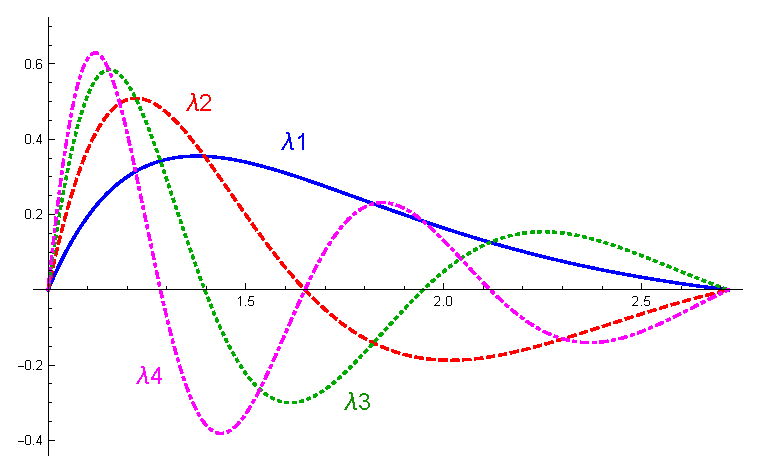
\includegraphics[scale=0.85]{Imagenes/Ejercicio_SL_01_Funciones.eps}
% \end{figure}
% \end{frame}

\end{document}